%! Author = itgramic
%! Date = 09.01.24

% Preamble
\chapter{Snapshots}
{
    \begin{flushleft}
        Um Snapshots für die Server zu machen, muss in die \Gls{VMware vSphere} ESXi-Site geöffnet werden:
    \end{flushleft}
    \begin{flushleft}
        \url{https://sks0174.sivc.first-it.ch/ui/}
    \end{flushleft}
    \begin{flushleft}
        Dort muss dann der entsprechende Server, in diesem Beispiel \texttt{sks0060}, gesucht werden und auf \texttt{Snapshots} gewechselt werden:
        \begin{figure}[H]
            \centering
            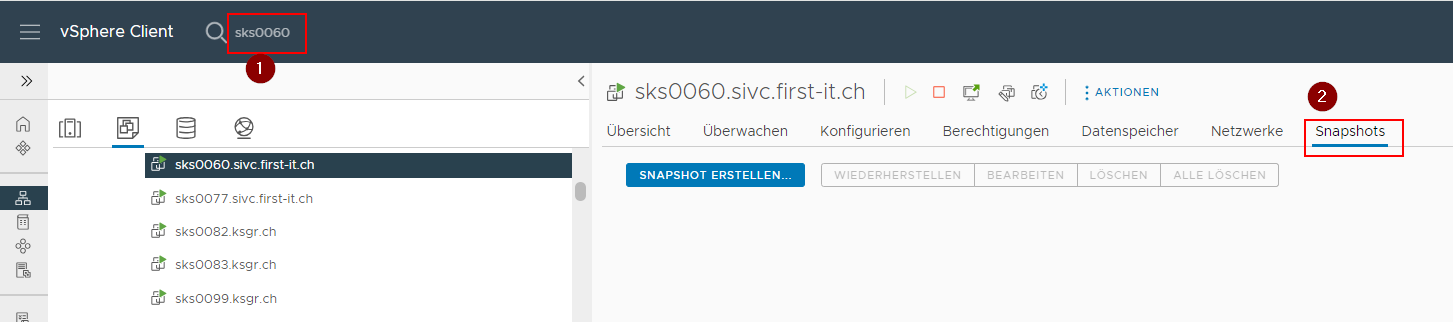
\includegraphics[width=1\linewidth]{source/snapshots/esxi_select_machine}
            \caption{ESXi - Maschine Suchen}
            \label{fig:esxi_select_machine}
        \end{figure}
    \end{flushleft}
    \begin{flushleft}
        Jetzt muss \texttt{SNAPSHOT ERSTELLEN...} geklickt werden.
        Wichtig ist, einen sprechenden Text in die Beschreibung zu hinteregen.
        \begin{figure}[H]
            \centering
            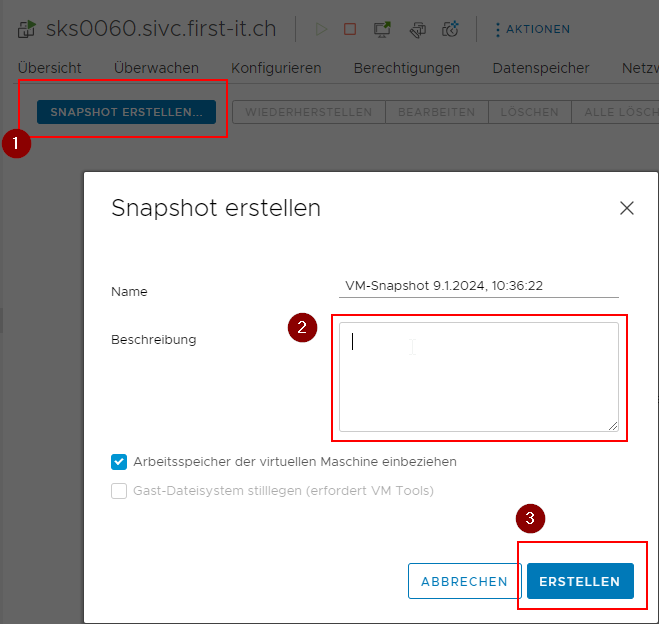
\includegraphics[width=0.5\linewidth]{source/snapshots/esxi_set_snapshot}
            \caption{ESXi - Snapshot erstellen}
            \label{fig:esxi_set_snapshot}
        \end{figure}
    \end{flushleft}
    \begin{flushleft}
        Die erstellung eines Snapshots kann bis zu meheren Minuten dauern.
        \begin{figure}[H]
            \centering
            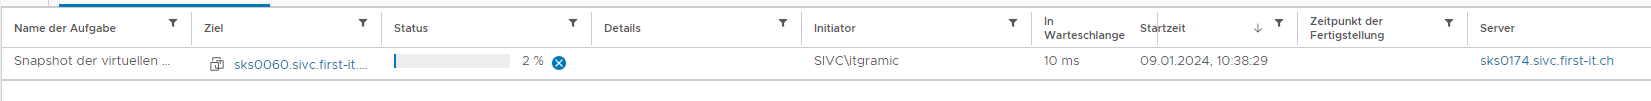
\includegraphics[width=1\linewidth]{source/snapshots/esxi_create_snapshote}
            \caption{ESXi - Snapshot wird erstellt}
            \label{fig:esxi_create_snapshote}
        \end{figure}
    \end{flushleft}
    \begin{flushleft}
        Ist der Snapshot erstellt, wird dies rückgemeldet:
        \begin{figure}[H]
            \centering
            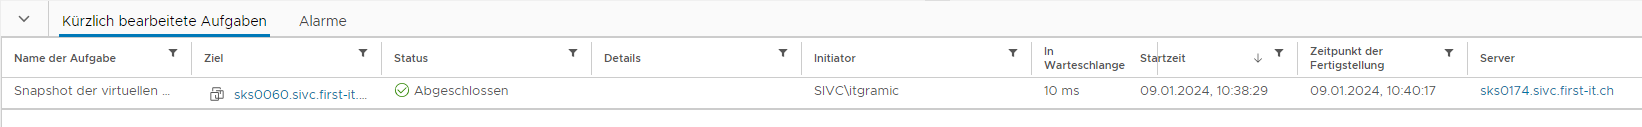
\includegraphics[width=1\linewidth]{source/snapshots/esxi_snapshot_created}
            \caption{ESXi - Snapshot wurde erstellt}
            \label{fig:esxi_snapshot_created}
        \end{figure}
    \end{flushleft}
}
{
    \begin{flushleft}
        Um einen Snapshot zu löschen, muss dieser ganz einfach angewählt werden\\
        und dann auf \texttt{LÖSCHEN} geklickt werden, wenn man nur einen Snapshot löschen will,
        \\oder \texttt{ALLE LÖSCHEN} wenn man alle Snpashots löschen will:
        \begin{figure}[H]
            \centering
            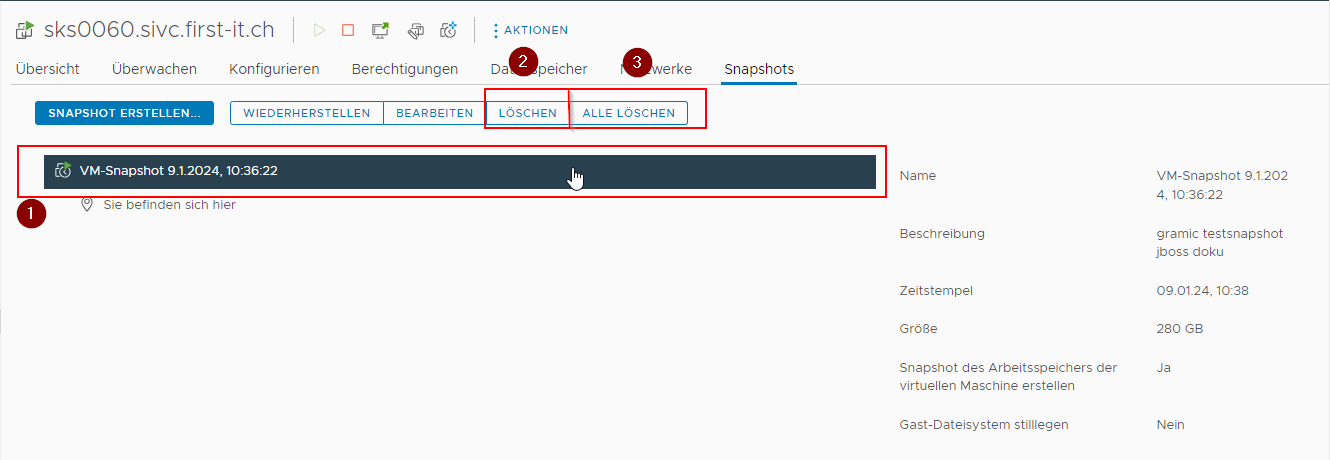
\includegraphics[width=0.5\linewidth]{source/snapshots/esxi_delete_snapshot}
            \caption{ESXi - Snapshot löschen}
            \label{fig:esxi_delete_snapshot}
        \end{figure}
    \end{flushleft}
    \begin{flushleft}
        Man muss aber bestätigen, dass man löschen möchte:
        \begin{figure}[H]
            \centering
            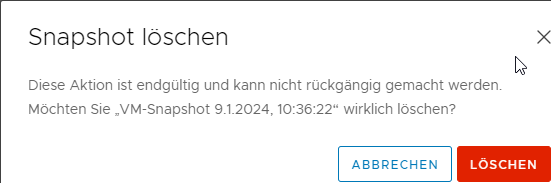
\includegraphics[width=0.5\linewidth]{source/snapshots/esxi_confirm_delete}
            \caption{ESXi - Snapshot löschen bestätigen}
            \label{fig:esxi_confirm_delete}
        \end{figure}
    \end{flushleft}
    \begin{flushleft}
        Auch das löschen kann eine weile dauern.
        Wurde der Snapshot gelöscht, wird auch das zurückgemeldet:
        \begin{figure}[H]
            \centering
            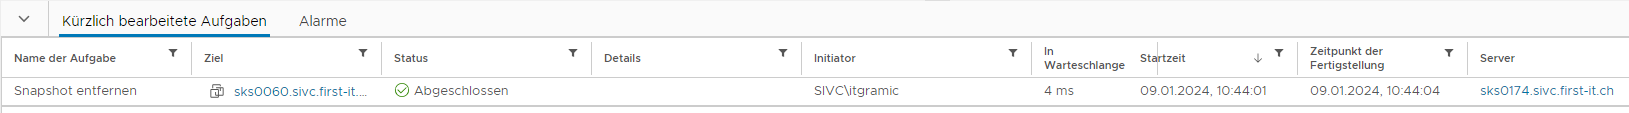
\includegraphics[width=0.5\linewidth]{source/snapshots/esxi_snapshot_deleted}
            \caption{ESXi - Snapshot gelöscht}
            \label{fig:esxi_snapshot_deleted}
        \end{figure}
    \end{flushleft}
    \begin{flushleft}
        \begin{mdframed}
            Bitte Snapshots Zeitnah löschen!\\
            Für längere Sicherungen ist das \Gls{VEEAM}-Backup vorhanden.\\
            Wird der Snapshot für länger als 3 Tage nicht gelöscht, so wird eine Meldung via Mail gesendet.
        \end{mdframed}
    \end{flushleft}
}